提案手法をデータセットの作成とモデルの作成から説明する。
すべての実装コードは筆者のgithubのレポジトリ (https://github.com/shinn1r0\\/endoscopic\_images2karte)にある。
実装には主にPythonを用い、深層学習フレームワークにはPytorchを使用した。
またプライバシー情報のためデータセット作成の元となる内視鏡画像と簡易カルテのデータ、それらから生成したデータセットは含まれていない。

\section{手法の分類}
本論文では図\ref{fig:methods}に示すように2つの手法を用いた。
\textcircled{\scriptsize 1}の手法は画像を個別にマルチラベルと関連付けで学習を行う。
\textcircled{\scriptsize 2}の手法は各患者ごとの全ての画像をまとめて三次元データとみなし、これをマルチラベルと関連付けで学習を行う。
そのため以下に続くデータセットとモデルの作成においても、それぞれ2種類用意した。

\textcircled{\scriptsize 1}の手法における学習手法は、患者単位の画像を1枚ずつモデルに入力し、出力された各ラベルとその患者のラベルから損失を計算し最適化を行うことを、画像の枚数回繰り返すという方法である。

\textcircled{\scriptsize 2}の手法における学習手法は、患者単位の画像を三次元データとしてモデルに入力し、出力された1つのラベルとその患者のラベルから損失を計算し最適化を行うという方法である。

学習手法は2つの手法で異なっているが、推論時はどちらの手法においても患者単位の画像を全て入力し、1人の患者のラベルを予測した。
\begin{figure}[htbp]
    \begin{center}
        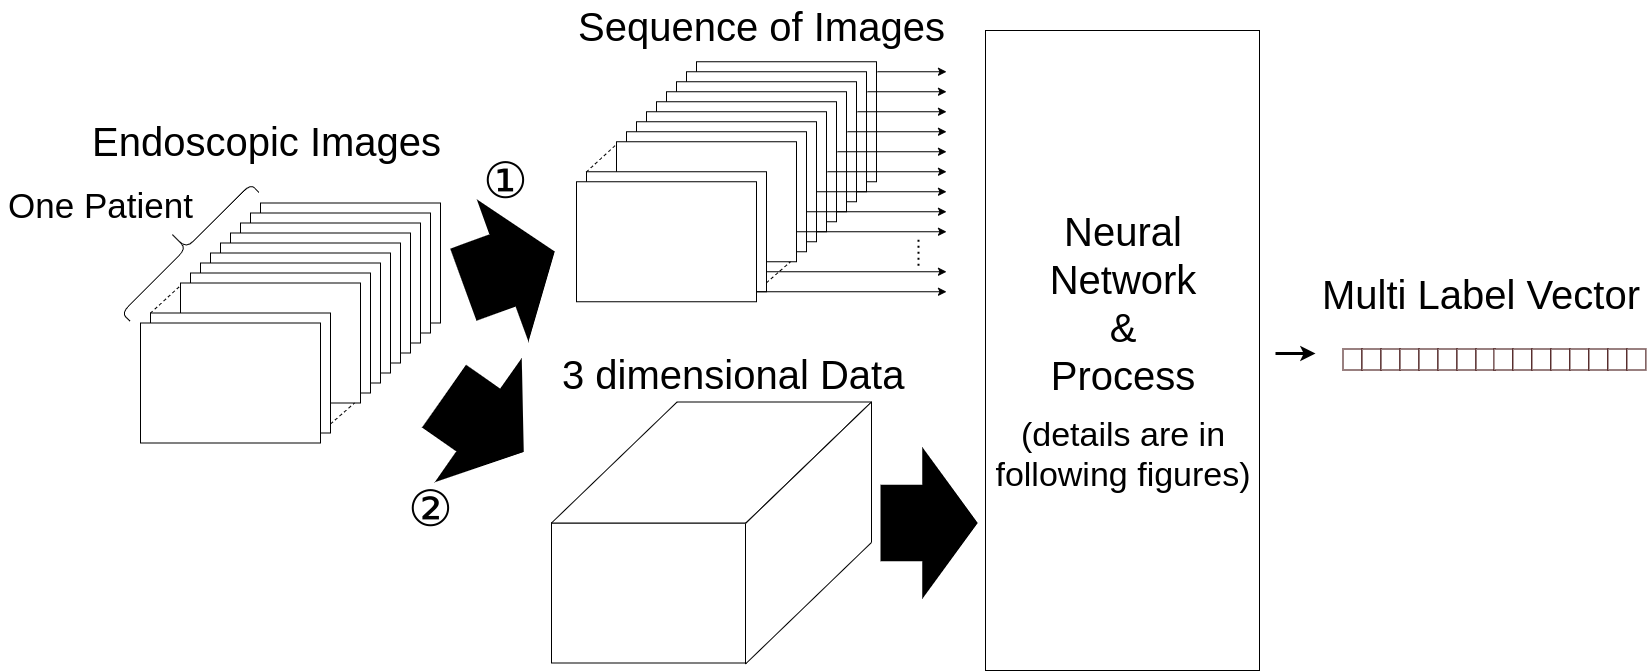
\includegraphics[width=135mm]{./fig/ieice4.png}
        \caption{提案手法}
        \label{fig:methods}
    \end{center}
\end{figure}

\section{データセットの作成}
2つの提案手法において、簡易カルテからのマルチラベル生成と各画像における処理は共通であるが、その後の処理はそれぞれの手法で異なる。
\subsection{簡易カルテからのマルチラベル生成}

\begin{figure}[htbp]
    \begin{center}
        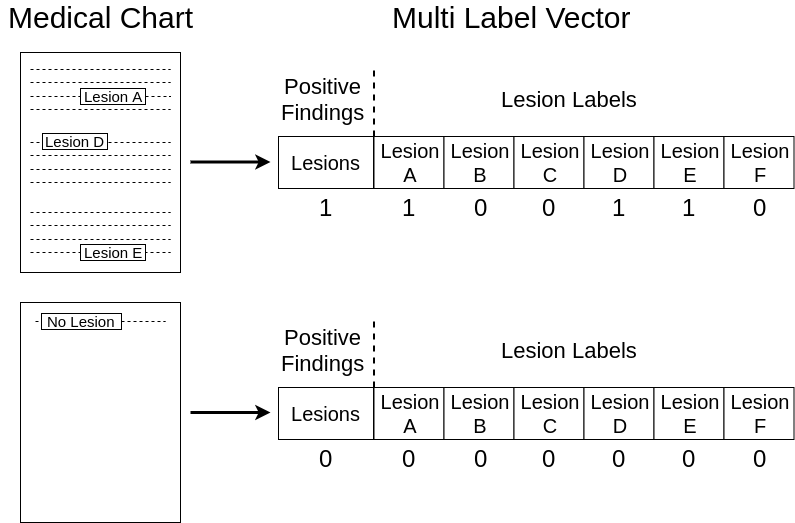
\includegraphics[width=130mm]{./fig/ieice1.png}
        \caption{データセット作成}
        \label{fig:multilabel}
    \end{center}
\end{figure}

簡易カルテからのマルチラベル生成を図\ref{fig:multilabel}に示す。
また手順は以下のように行った。

\begin{enumerate}
    \item すべて異常なしの患者を抽出
    \item 簡易カルテ内の質的診断を言語処理
    \item 処理後の内容を全ての患者でまとめてカテゴリー化
    \item 頻出病名カテゴリー選択
    \item 各患者ごとにマルチラベル生成
    \item マルチラベルのone-hotベクトル化
\end{enumerate}

詳細を以下に述べる。

 1.では簡易カルテ内の全ての行で異常なしとなっている患者を抜き出し、 2.から 4.の処理には通していない。

 2.では簡易カルテ内の質的診断の項目のみを取り出し、各行あたりに言語処理を行った。

この言語処理では文書であったり単語や数値の羅列であったりする質的診断をまず単語の系列データへと変換した。
次にこれらを形態素解析\cite{MeCab}や事前に用意した病名リストを用いた検索などを通して病名を表す単語とそれらに付随する情報を示す単語を抽出した。
その際に複雑な付随情報を持つような病名は固有の処理を加えている。
これらの処理の詳細を\ref{sec:nl}に示す。

これにより簡易カルテの質的診断の項目では、各行が、先頭に病名単語があり、その後に付加情報単語が続く形式になる。

3.では 2.の処理後の内容を全ての患者を通して集計し、同じ単語を同じラベル付けをして辞書に格納した。 

4.では辞書内で出現回数を計測し、指定した回数以上のラベルを頻出病名ラベルとして決定した。
本研究ではすべて頻出病名を15個に設定した。

 5. 6.では各患者ごとにone-hot化したマルチラベルを生成した。
マルチラベルの1番目のラベルには異常が一つでもある患者は1を、それ以外の患者は0が格納されている。
これには 1.で抽出した情報を用いた。
マルチラベルの2番目以降のラベルには頻出病名ラベルがある。 
2.から 4.で作成した情報を元に、各患者の質的診断の項目に頻出病名が存在する場合は1を、存在しない場合は0が格納されている。

\subsection{言語処理の詳細}
\label{sec:nl}
簡易カルテからマルチラベルを生成する際に行った言語処理の詳細を述べる。
\subsubsection{言語処理の流れ}
\begin{enumerate}
    \item 入力された文の中で半角が存在する文字はすべて半角に変換する。
    \item 表\ref{tb:nl1}にある記号や特定の数字や単語で文を単語列に分割する。
        \begin{table}[htbp]
            \caption[]{分割の区切りに利用した記号や特定の数字や単語や文}
            \label{tb:nl1}
            \centering
            \normalsize
            \begin{tabular}{c|c} \hline
                記号 & 特定の数字や単語や文 \\ \hline \hline
                句点 & 先頭にある数字 \\ \hline
                読点 & に対して \\ \hline
                カンマ & による \\ \hline
                ピリオド & にて \\ \hline
                中点 & \\ \hline
                コロン & \\ \hline
                セミコロン & \\ \hline
                スペース & \\ \hline
                全角スペース & \\ \hline
                タブ (\textbackslash t) & \\ \hline
                改行 (\textbackslash n, \textbackslash r, \textbackslash rn) & \\ \hline
            \end{tabular}
        \end{table}
    \item 単語列の中で単語なしの要素があれば削除する。
    \item 表\ref{tb:nl2}にある頻出する表記ゆれに対応する。
        \begin{table}[htbp]
            \caption[]{表記ゆれへの対応}
            \label{tb:nl2}
            \centering
            \normalsize
            \begin{tabular}{c|c} \hline
                表記ゆれ & 統一後の表記 \\ \hline \hline
                疑う所見なし & \\
                示唆する所見なし & 所見なし \\
                所見なし & \\ \hline
                CRTX & \\
                CRTx & CRTx後 \\
                CRTx後 & \\ \hline
                疑う & 疑い \\
                疑い & \\ \hline
                ELPS後 & ELPS後瘢痕 \\
                ELPS後瘢痕 & \\ \hline
            \end{tabular}
        \end{table}
    \item 度合いや付加状態を取り出す。 \\
        ・軽度 \\
        ・重度 \\
        ・疑い \\
        ・術後
    \item 大きさを取り出す。 \\
        ・正規表現 ([0-9]* \textbackslash .*[0-9]*[a-z]*m[a-z]*) で取り出す。
    \item 表\ref{tb:nl3}にある特定の病名を優先的に取り出す。
        \begin{table}[htbp]
            \caption[]{優先的に取り出す病名}
            \label{tb:nl3}
            \centering
            \normalsize
            \begin{tabular}{|c|} \hline
                病名 \\ \hline \hline
                食道癌 \\ \hline
                マロリーワイス症候群 \\ \hline
                ヘルニア \\ \hline
                ポリープ \\ \hline
                カンジダ症 \\ \hline
                ヨード不染 \\ \hline
                咽頭喉頭炎 \\ \hline
                十二指腸炎 \\ \hline
                静脈拡張 \\ \hline
                潰瘍 \\ \hline
                リンパ腫 \\ \hline
                ペンタサ \\ \hline
            \end{tabular}
        \end{table}
    \item 表\ref{tb:nl4}にある特定の病名を付加情報とともに取り出す。
        \begin{table}[htbp]
            \caption[]{付加情報とともに優先的に取り出す病名}
            \label{tb:nl4}
            \centering
            \normalsize
            \begin{tabular}{c|c} \hline
                病名 & 付加情報 \\ \hline \hline
                         & RAC \\ \cline{2-2}
                         & 胃底腺ポリープ \\ \cline{2-2}
                         & 稜線状発赤 \\ \cline{2-2}
                慢性胃炎 & 扁平隆起 \\ \cline{2-2}
                         & ヘマチン付着 \\ \cline{2-2}
                         & 地図状発赤 \\ \cline{2-2}
                         & 色調逆転現症 \\ \hline
                逆流性食道炎 & grade \\ \cline{2-2}
                             & LA \\ \hline
                胃術後 & 摘出部分(全部・上半分・下半分) \\ \cline{2-2}
                       & 接続方法 \\ \hline
            \end{tabular}
        \end{table}
    \item 残りの要素を付加情報として追加する。
\end{enumerate}
すべての要素追加時に以下の品詞を含む要素を除外した。 \\
    ・助詞 \\
    ・接続詞 \\
    ・接頭辞 \\
    ・助動詞 \\
    ・副詞可能名詞

\subsection{各画像における処理}
実際の画像サイズには$1000 \times 870$ピクセル、$640 \times 480$ピクセルなど複数ある。
そこですべての画像は$256 \times 256$ピクセルにサイズ変更した。
サイズ変更はPytorch\cite{Pytorch}のResize関数を用いた。
その後画像のRGBチャンネルそれぞれを正規化した。
正規化のパラメータはRが平均0.485、標準偏差0.229、Gが平均0.456、標準偏差0.224、Bが平均0.406、標準偏差0.225に設定した。
これらの値はすべて深層学習フレームワークのPytorch\cite{Pytorch}で推奨されている値である。
\subsection{データセット分割}
2つの手法に合わせてデータセットを2つ用意した。
それぞれのデータセットは訓練データ、検証データ、テストデータに分割した。
\begin{itemize}
    \item 画像を個別に入力する手法\\
この手法では、学習に用いる訓練データと検証データは画像を全患者に渡ってランダムにし、それぞれをマルチラベルと関連付けした。
それに対して、テストでは患者単位での予測になるために、テストデータは患者単位で検査順に並んだ画像を系列データとしてマルチラベルと関連付けした。
    \item 画像を患者ごとにまとめて入力する手法\\
この手法では、学習とテストに用いる全てのデータを患者単位でまとめた。
データは検査順に並べた画像を時間軸で連結させ、三次元データとし、それぞれマルチラベルと関連付けした。
\end{itemize}

\section{モデルの作成}
2つの手法に合わせてモデルも2つ用意した。
どちらのモデルでも残差構造を持っていて、表現力の大きい多層のCNNを用いている。
モデルの選択はPytorchで安定的に良い性能があるとされていて、用いられることが多いものを参考にした。
\begin{itemize}
    \item 画像を個別に入力する手法\\
この手法では残差構造を持つCNN\cite{CNN}で最も一般的なResNet\cite{ResNet}を発展させたDenseNet\cite{DenseNet}を用いた。
残差構造では、従来のネットワークでは同じ深さの層では同じ大きさの特徴しか抽出できなかったのに対して、ショートカットを用いることで同じ深さの層でも異なる大きさの特徴を抽出できるようになっている。
ResNet\cite{ResNet}はネットワークの主要部分で畳み込みを行って、ショートカット部分でその畳み込みを飛ばす構造をしている。
DenseNet\cite{DenseNet}では主要部分では畳み込みを行わず、分岐した部分に設置したDense Blockによって畳み込みを行い、その出力が主要部分で合流する構造をしている。
これによりResNet\cite{ResNet}より少ないパラメータ数で効率良く特徴抽出ができることが確認されている。

Dense Blockの式は複数の層の集合からなり、第l層の出力を\mbox{\boldmath $x_l$}とすると、Dense Block全体での第l層の出力は以下の式で表される。
\begin{equation}
    \mbox{\boldmath $x_l$} = H_l([\mbox{\boldmath $x_0$}, \mbox{\boldmath $x_1$}, … , \mbox{\boldmath $x_{l-1}$}])
\end{equation}

ここで$H_l$はバッチ正規化、ReLU活性化関数、$3 \times 3$の畳み込み層からなる合成関数である。
それぞれの詳細を以下に述べる。

\begin{itemize}
    \item バッチ正規化

    \begin{equation}
         y = \frac{x - E[x]}{\sqrt{Var[x] + \epsilon}} * \beta + \gamma
    \end{equation}
    $\beta$と$\gamma$はパラメータで通常は1と0である。
    $E[x]$は平均値、$Var[x]$は分散値である。また$\epsilon$は任意の正の実数である。

    \item ReLU活性化関数

    \begin{equation}
         ReLU(x) = max(0, x)
    \end{equation}
    $max$は最大値である。

    \item $3 \times 3$の畳み込み層

    バッチサイズを$N$、チャンネルを$C$、画像の高さを$H$、幅を$W$とする。
入力チャンネルを$C_{in}$、入力画像の高さを$H_{in}$、幅を$W_{in}$とし、出力チャンネルを$C_{out}$、出力画像の高さを$H_{out}$、幅を$W_{out}$としたとき、入力テンソルの形式が$(N, C_{in}, H_{in}, W_{in})$、出力テンソルの形式が$(N, C_{out}, H_{out}, W_{out})$となる。
このとき$i$番目のバッチ$N_i$の$j$番目のチャンネル$C_{out_j}$の出力画像は以下の式で表される。

    \begin{equation}
        out(N_i, C_{out_j}) = bias(C_{out_j}) + \sum_{k=0}^{C_{in} - 1} weight(C_{out}, k) * input(N_i, k)
    \end{equation}
    またこのとき、$H_{out}$と$W_{out}$は以下のように計算される。
畳み込み幅 (kernel\_size)を$\bm{K}$、余白 (padding)を$\bm{P}$、畳み込みの移動幅 (stride)を$\bm{S}$、畳み込みの際にピクセル間に取る空白 (dilation)を$\bm{D}$を長さ2の一次元配列で設定する。
一つ目の要素に画像の縦に関する設定が、二つ目の要素に画像の横に関する設定が格納されている。
このとき、畳み込み幅 (kernel\_size)の$i$番目の要素は$k_i$、余白 (padding)の$i$番目の要素は$p_i$、畳み込みの移動幅 (stride)の$i$番目の要素は$s_i$、畳み込みの際にピクセル間に取る空白 (dilation)の$i$番目の要素は$d_i$となる。

    \begin{equation}
        H_{out} = \frac{H_{in} + 2 \times p_0 - d_0 \times (k_0 - 1) - 1}{s_0} + 1
    \end{equation}

    \begin{equation}
        W_{out} = \frac{W_{in} + 2 \times p_1 - d_1 \times (k_1 - 1) - 1}{s_1} + 1
    \end{equation}

\end{itemize}

    \item 画像を患者ごとにまとめて入力する手法\\
この手法では画像を連結し、時系列データを三次元データとして入力するため、CNNを三次元に拡張した3D-CNNを用いた。
3D-CNNの中でも現在最も良い性能を持っている3D-ResNet\cite{3D_ResNet}を選択した。
\end{itemize}

\begin{figure}[htbp]
    \begin{center}
        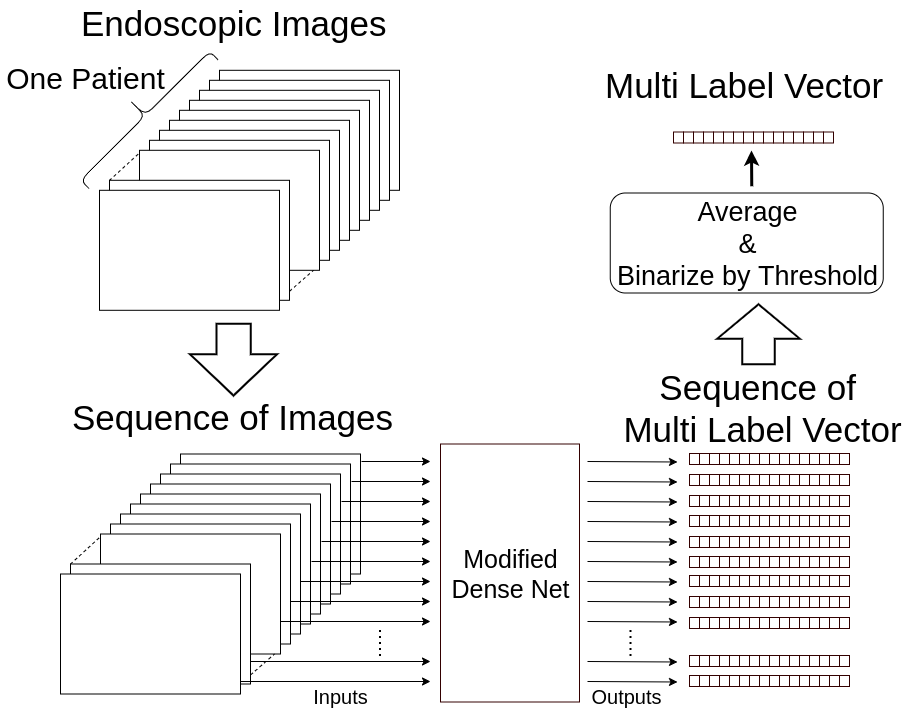
\includegraphics[width=122mm]{./fig/ieice2.png}
        \caption{DenseNetを使った手法}
        \label{fig:densenet}
    \end{center}
\end{figure}

\begin{figure}[htbp]
    \begin{center}
        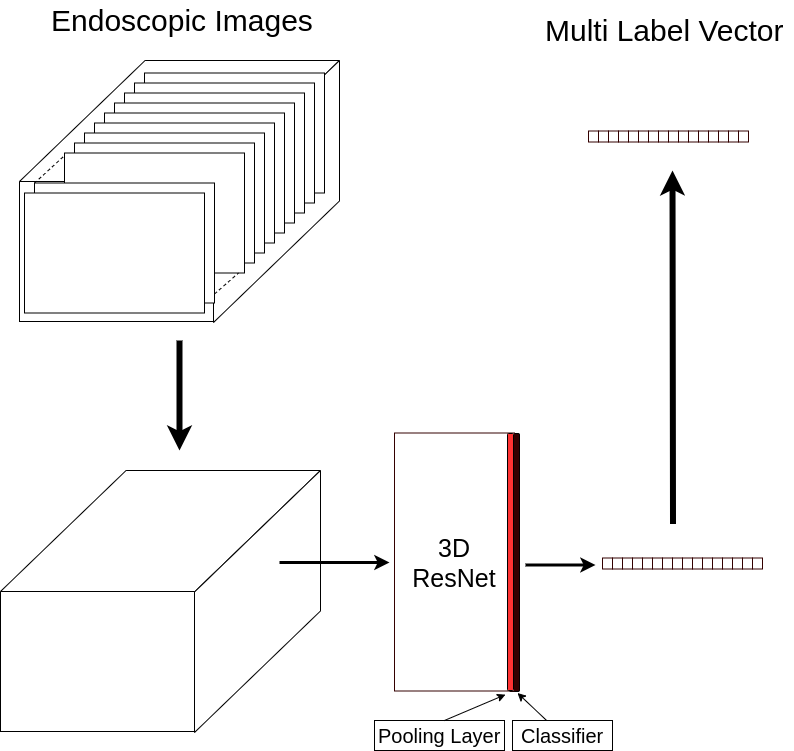
\includegraphics[width=122mm]{./fig/ieice3.png}
        \caption{3D-ResNetを使った手法}
        \label{fig:3d_resnet}
    \end{center}
\end{figure}

\newpage
\subsection{DenseNetのチューニング}
\label{sec:densenet}
DenseNetのチューニングをし、複数のモデルを用意した。
これを図\ref{fig:densenet}に示す。
全てのモデルにおいて共通していることは、特徴抽出部分をそのまま用いていることと、分類器部分の最終層のニューロン数をマルチラベルのクラス数と合わせていることである。
これに加えて分類器部分を変更したものも用意した。
通常は一層の全結合層のみの構造であったが、複数の全結合層とバッチ正規化とドロップアウトをからなる構造に変更した。
これを分類器拡張とし、分類器拡張ありと分類器拡張なしの2パターンを用意した。
マルチラベル予測においては、抽出した特徴の組み合わせが1つのラベルの予測よりも複雑になる。
そのため分類器においても深層の構造を用いた。
また今回の実験ではより複雑な特徴にも対応するために、層の数の異なる2つのDenseNetで学習した。
それぞれDenseNet121\cite{DenseNet}とDenseNet161\cite{DenseNet}というモデルを用いた。
このため合わせて4パターンで実験を行った。

DenseNet121において分類器拡張をしていないものをモデル1とし、付録の図\ref{fig:model11}に示す。

DenseNet121において分類器拡張をしたものをモデル2とし、付録の図\ref{fig:model12}に示す。

DenseNet161において分類器拡張をしていないものをモデル3とし、付録の図\ref{fig:model13}に示
す。

DenseNet161において分類器拡張をしたものをモデル4とし、付録の図\ref{fig:model14}に示す。

\subsection{3D-ResNetのチューニング}
\label{sec:resnet3d}
3D-ResNetのチューニングをし、複数のモデルを用意した。
これを図\ref{fig:3d_resnet}に示す。
特徴抽出部分の最終層において、通常では平均プーリングをして特徴を合算している。
その際に特徴が損失する恐れがあったため、これを最大プーリングに置き換えたものも用意した。
また分類器部分でもDenseNetのときと同じように分類器拡張ありと分類器拡張なしの2つのパターンを用意した。
これは一層の全結合層のみのものと、複数の全結合層とバッチ正規化とドロップアウトからなる構造のものである。
このため合わせて4パターンで実験を行った。

3D-ResNetで平均プーリングを用いて分類器をしていないものをモデル1とし、付録の図\ref{fig:model21}に示す。

3D-ResNetで平均プーリングを用いて分類器をしたものをモデル2とし、付録の図\ref{fig:model22}に示す。

3D-ResNetで最大プーリングを用いて分類器をしていないものをモデル3とし、付録の図\ref{fig:model23}に示す。

3D-ResNetで最大プーリングを用いて分類器をしたものをモデル4とし、付録の図\ref{fig:model24}に示す。
